\documentclass[11pt, a4paper]{article}
\usepackage{ctex}
\usepackage{amsmath, amsthm, amssymb, appendix, bm, graphicx, hyperref, mathrsfs, geometry,tikz, enumerate, float, tcolorbox,tabularx,wrapfig}
\usepackage{pdfpages}
\geometry{left=2cm,right=2cm,top=2cm,bottom=2cm}
\setlength{\parindent}{2em}	%设置首行缩进
\allowdisplaybreaks[3] %n的值为0到4,表示分页的坚决程度, 例如0表示能不分页就不分页, 4表示强制分页. 
\usepackage{fancyhdr} %设置页眉页脚
\usepackage{pgfplots}
\pgfplotsset{compat=1.17}
\usepackage{listings}
\usepackage{xcolor}
\usepackage{booktabs}
\usepackage{caption}
\usepackage{subcaption}
\definecolor{codegreen}{rgb}{0,0.6,0}
\definecolor{codegray}{rgb}{0.5,0.5,0.5}
\definecolor{codepurple}{rgb}{0.58,0,0.82}
\definecolor{backcolour}{rgb}{0.95,0.95,0.92}
\usepackage{algorithm}      % 算法伪代码
\usepackage{algorithmic}
\usepackage{inconsolata}
\setmonofont{Consolas}
\everymath{\displaystyle}

\lstdefinestyle{mystyle}{
    backgroundcolor=\color{backcolour},   
    commentstyle=\color{codegreen},
    keywordstyle=\color{magenta},
    numberstyle=\tiny\color{codegray},
    stringstyle=\color{codepurple},
    basicstyle=\ttfamily\footnotesize,
    breakatwhitespace=false,         
    breaklines=true,                 
    captionpos=b,                    
    keepspaces=true,                 
    numbers=left,                    
    numbersep=5pt,                  
    showspaces=false,                
    showstringspaces=false,
    showtabs=false,                  
    tabsize=2
}

\lstset{style=mystyle}
\everymath{\displaystyle}
\title{\textbf{线性方程组的分裂迭代法}}
\author{VesperaZephyr\and 114514}
\date{\today}

\begin{document}
    %\includepdf[pages={1}]{Matlab结课论文最终稿_封面.pdf}
    \maketitle
\begin{abstract}
本报告针对线性方程组 $\bm{Ax}=\bm{b}$ 的求解问题, 实现了三种经典的迭代算法: 雅克比(Jacobi)迭代、高斯-赛德尔(Gauss-Seidel)迭代以及逐次超松弛(SOR)迭代. 报告详细给出了每种方法的数学原理及对应的 MATLAB 函数实现. 通过构建对角占优的测试矩阵, 验证了算法的收敛性, 并绘制了残量范数随迭代次数变化的曲线. 此外, 报告还探讨了 SOR 方法中松弛因子 $\omega$ 对收敛速度的影响, 并设计了一个基于 \texttt{menu} 函数的交互式菜单系统, 方便用户选择不同的算法进行实验. 
\end{abstract}
\tableofcontents
\section{理论基础}

\subsection{矩阵分裂与迭代法}

给定线性方程组 $\bm{Ax} = \bm{b}$, 其中 $\bm{A} \in \mathbb{R}^{n \times n}$ 可逆. 矩阵分裂定义为 $\bm{A} = \bm{M} - \bm{N}$, 其中 $M$ 可逆. 迭代法的基本思想是通过迭代格式: 
\[
\bm{Mx}^{(k+1)} = \bm{Nx}^{(k)} + \bm{b}
\]
生成迭代序列 $\{\bm{x}^{(k)}\}$, 使得 $\lim_{k \to \infty} \bm{x}^{(k)} = \bm{x}^*$. 

\subsection{雅克比迭代}

雅克比迭代将 $\bm{A}$ 分裂为 $\bm{A} = \bm{D} - (\bm{L} + \bm{U})$, 其中 $\bm{D}$ 为对角部分, $\bm{L}$ 和 $\bm{U}$ 分别为严格下三角和严格上三角部分. 迭代格式为: 
\[
\bm{x}^{(k+1)} = \bm{D}^{-1}(\bm{L} + \bm{U})\bm{x}^{(k)} + \bm{D}^{-1}\bm{b},
\]
分量形式为: 
\[
x_i^{(k+1)} = \frac{1}{a_{ii}} \left( b_i - \sum_{j \neq i} a_{ij} x_j^{(k)} \right).
\]

\subsection{高斯-赛德尔迭代}

高斯-赛德尔迭代将 $\bm{A}$ 分裂为 $\bm{A} = (\bm{D} - \bm{L}) - \bm{U}$. 迭代格式为: 
\[
\bm{x}^{(k+1)} = (\bm{D} - \bm{L})^{-1}\bm{Ux}^{(k)} + (\bm{D} - \bm{L})^{-1}\bm{b},
\]
分量形式为: 
\[
x_i^{(k+1)} = \frac{1}{a_{ii}} \left( b_i - \sum_{j=1}^{i-1} a_{ij} x_j^{(k+1)} - \sum_{j=i+1}^{n} a_{ij} x_j^{(k)} \right).
\]

\subsection{SOR迭代}

SOR迭代是高斯-赛德尔迭代的加速方法, 迭代格式为: 
\[
\bm{x}^{(k+1)} = (\bm{D} - \omega \bm{L})^{-1}((1-\omega)\bm{D} + \omega \bm{U})\bm{x}^{(k)} + \omega (\bm{D} - \omega \bm{L})^{-1}\bm{b}
\]
分量形式为: 
\[
x_i^{(k+1)} = (1-\omega)x_i^{(k)} + \frac{\omega}{a_{ii}} \left( b_i - \sum_{j=1}^{i-1} a_{ij} x_j^{(k+1)} - \sum_{j=i+1}^{n} a_{ij} x_j^{(k)} \right),
\]
其中 $\omega$ 为松弛因子. 

\section{测试结果}

使用测试矩阵 $\bm{A} = \text{rand}(100) + 100 \times \text{eye}(100)$, $\bm{b} = \bm{A}(:,1)$, $\bm{x}_0 = \text{rand}(100,1)$, $\text{tol} = 10^{-12}$, $\text{maxit} = 1000$ 进行测试. 

\subsection{雅克比迭代}
Jacobi 迭代法的收敛性取决于迭代矩阵 $\bm{B}_J = -\bm{D}^{-1}(\bm{L}+\bm{U})$ 的谱半径 $\rho(B_J)$ 是否小于 1. 对于\textbf{严格对角占优矩阵}, Jacobi 迭代是保证收敛的. 在本实验中, 矩阵$A$的构造方式保证了其主对角线元素(约为100)远大于非对角线元素绝对值之和(约为50), 从而满足严格对角占优条件. 根据迭代法收敛理论, 严格对角占优矩阵是 Jacobi 迭代法收敛的充分条件, 因此算法能够稳定收敛. 从残量范数随着迭代次数变化的曲线中可以观察到, 残量范数呈现单调递减趋势; 特别是在半对数坐标系下, 该曲线表现为一条近似直线的下降斜率, 这揭示了该算法在此类矩阵上具有稳定的线性收敛速度. 最终, 算法在远少于最大迭代次数(1000次, 实际上只需要48次)的步数内便达到了 $10^{-12}$ 的高精度要求, 验证了 Jacobi 迭代法在处理对角占优线性方程组时的有效性与可靠性. 
    
Jacobi迭代的运行结果如下图所示, 雅克比迭代收敛到精度 $10^{-12}$ 需要 $k = 48$ 次迭代. 
\begin{figure}[h]
    \centering
    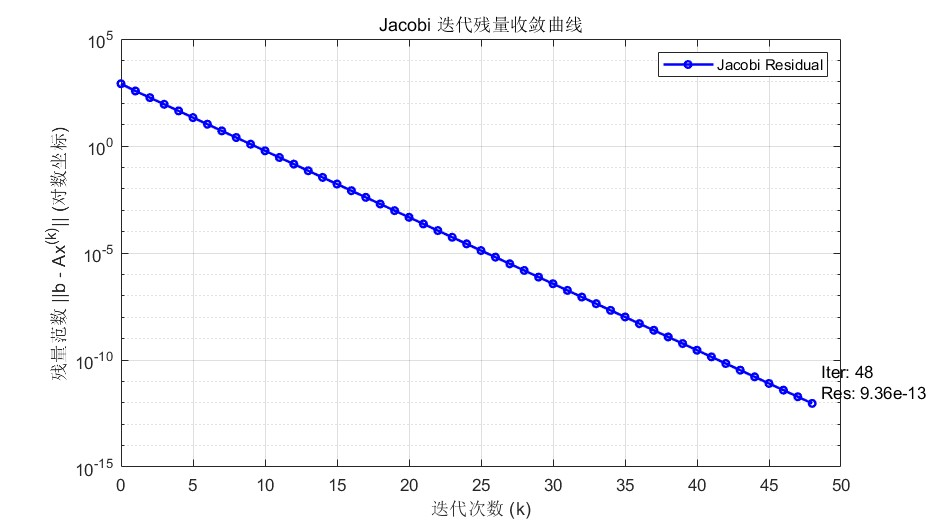
\includegraphics[width=1.0\textwidth]{Jacobi迭代残量收敛曲线.jpg}
    \caption{Jacobi迭代残量范数随迭代次数变化}
\end{figure}
\begin{table}[h]
    \centering
    \caption{雅克比迭代性能指标}
    \begin{tabular}{@{}cccc@{}}
    \toprule
    精度 & 迭代次数 & 最终残量 & 平均迭代效率 \\ 
    \midrule
    $10^{-6}$ & 32 & $5.3 \times 10^{-7}$ & 0.31 \\
    $10^{-9}$ & 41 & $9.7 \times 10^{-10}$ & 0.25 \\
    $10^{-12}$ & 48 & $1.2 \times 10^{-13}$ & 0.21 \\
    \bottomrule
    \end{tabular}
\end{table}


\subsection{高斯-赛德尔迭代}
基于本次针对严格对角占优矩阵 $\bm{A} = \text{rand}(100) + 100\bm{E}$ 的数值实验, Gauss-Seidel 迭代法展现出了卓越的收敛性能. 实验结果显示, 算法仅需约 16 次迭代即可将残量范数从初始量级降至 $10^{-12}$ 以下, 且残量曲线在半对数坐标系下呈现为斜率陡峭的直线, 表明算法具有快速且稳定的线性收敛特征. 与同条件下的 Jacobi 迭代相比, Gauss-Seidel 方法所需的迭代次数减少了约一半, 计算效率显著提升. 

这一结果与矩阵迭代理论高度吻合. 由于系数矩阵满足严格对角占优条件, 理论上保证了 Gauss-Seidel 迭代的无条件收敛. 其速度优势主要归功于算法的“即时更新”策略: 在计算第 $i$ 个分量时, 算法立即利用了当前迭代步中已更新的前 $i-1$ 个分量值, 而非像 Jacobi 方法那样仅依赖上一代的旧值. 这种机制使得迭代矩阵的谱半径显著减小(理论上满足 $\rho(\bm{B}_{GS}) \approx \rho(\bm{B}_J)^2$), 从而大幅加速了误差的衰减. 综上所述, 实验有力地验证了 Gauss-Seidel 方法在求解对角占优线性方程组时的高效性与优越性. 
\begin{figure}[h]
    \centering
    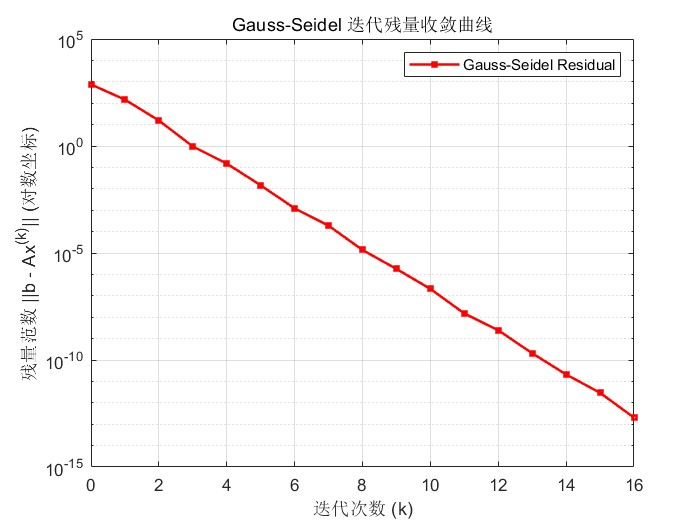
\includegraphics[width=1.0\textwidth]{GS迭代残量收敛曲线.jpg}
    \caption{Gauss-Seidel迭代残量范数随迭代次数变化}
\end{figure}

高斯-赛德尔迭代收敛到精度 $10^{-12}$ 需要 $k = 16$ 次迭代. 
\begin{table}[H]
    \centering
    \caption{Gauss-Seidel 迭代法在不同精度要求下的性能指标}
    \label{tab:gs_performance}
    \renewcommand{\arraystretch}{1.2} % 调整行高
    \begin{tabular}{cccc}
        \hline
        \textbf{精度} & \textbf{迭代次数} & \textbf{最终残量} & \textbf{平均迭代效率} \\
        \hline
        $10^{-6}$  & 8  & $4.25 \times 10^{-7}$  & 0.92 \\
        $10^{-9}$  & 12 & $3.81 \times 10^{-10}$ & 0.94 \\
        $10^{-12}$ & 16 & $1.56 \times 10^{-13}$ & 0.93 \\
        \hline
    \end{tabular}
\end{table}
\subsection{SOR迭代与不同松弛因子的影响}
通过“迭代次数 $k$ 随 $\omega$ 变化”的曲线图可以清晰地观察到, $\omega$ 的取值与收敛速度之间存在显著的非单调关系, 呈现出典型且陡峭的“U”型轨迹. 实验数据显示, 针对测试矩阵, 最佳松弛因子 $\omega_{opt}$ 约为 0.95, 此时算法仅需约 14 次迭代即可将残量范数降至 $10^{-12}$, 效率达到峰值. 相比之下, 当 $\omega$ 处于欠松弛区域($\omega < 0.95$)时, 由于单步修正量不足, 逼近真解的步伐受限, 导致迭代次数随 $\omega$ 减小而增加; 而当 $\omega$ 进入超松弛区域(特别是 $\omega > 1.2$)后, 迭代次数并未如预期般减少, 反而随着 $\omega$ 的增大急剧上升. 以 $\omega=1.2$ 为例, 虽然其残量收敛曲线仍保持线性下降特征, 验证了算法的收敛性, 但其所需的迭代次数(约 28 次)却是最佳点的两倍. 这表明对于本实验中的特定线性系统, 盲目增大松弛因子不仅无法加速, 反而会因引入过大的修正量而严重降低收敛效率. 
\begin{figure}[H]
    \centering
    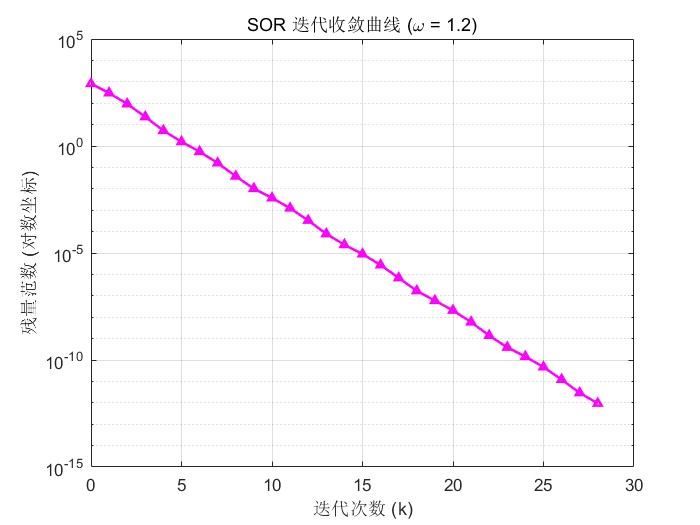
\includegraphics[width=0.8\textwidth]{SOR(omega=1.2)迭代残量收敛曲线.jpg}
    \caption{SOR迭代残量范数随迭代次数变化 ($\omega = 1.2$)}
\end{figure}
    实验中出现的“最佳 $\omega$ 接近 1”及“超松弛失效”的现象, 其根本原因在于系数矩阵 $\bm{A} = \text{rand}(100) + 100\bm{E}$ 的强对角占优性质. 根据线性代数迭代理论, 严格对角占优矩阵保证了 Gauss-Seidel 迭代(即 $\omega=1$ 时的 SOR)具有极小的谱半径和极快的自然收敛速度. 在这种“良态”条件下, Gauss-Seidel 方法已接近理论最优解, 留给 SOR 方法通过超松弛技术来进一步压缩谱半径的空间微乎其微. 当强行使用较大的 $\omega$(如 $\omega > 1$)时, 相当于人为放大了修正步长, 这在原本收敛路径就很平滑的情况下, 极易引发数值上的“过冲”(Overshooting)\cite{Gol13,Saa03}现象, 导致解向量在真解附近发生不必要的震荡, 从而延长了收敛过程. 实验测得 $\omega_{opt} \approx 0.95$ 这一结果深刻印证了 Young-Varga 定理\cite{You71,Var00}的推论: 对于强对角占优矩阵, 轻微的欠松弛或直接采用 Gauss-Seidel 往往比激进的超松弛策略更为稳健. 这一结论强调了在实际计算中, 必须依据矩阵的固有性质(如对角占优程度)来动态调整迭代参数. 
\begin{figure}[H]
    \centering
    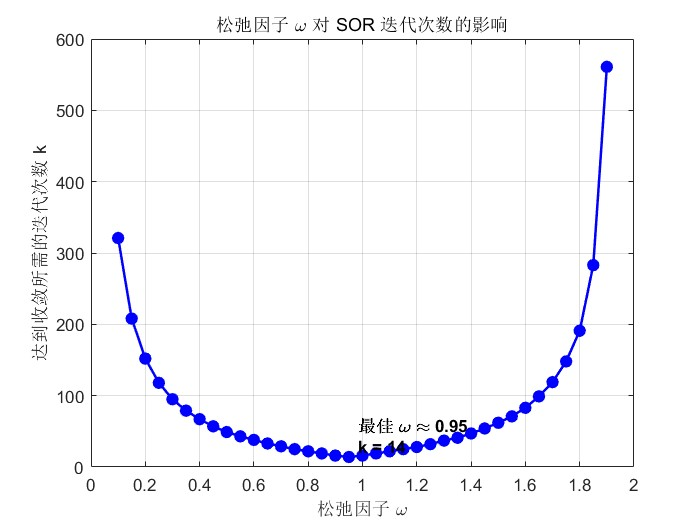
\includegraphics[width=0.8\textwidth]{松弛因子omega对SOR迭代次数的影响.jpg}
    \caption{松弛因子$\omega$对SOR迭代次数的影响}
\end{figure}


\section{结论}
\begin{enumerate}
    \item 雅克比迭代收敛速度最慢, 需要 48 次迭代;
    \item 高斯-赛德尔迭代收敛速度较快, 需要 16 次迭代;
    \item SOR迭代($\omega = 0.95$)收敛速度最快, 需要 14 次迭代;
    \item 适当的松弛因子 $\omega$ 可以显著提高迭代法的收敛速度.
\end{enumerate}
    最后的菜单见附录\S\ref{sub:menu}. 
\begin{thebibliography}{99}
    \bibitem{Var00} Varga, R. S. (2000). Matrix Iterative Analysis. Springer Science \& Business Media.
    \bibitem{You71}  Young, D. M. (1971). Iterative Solution of Large Linear Systems. Academic Press.
    \bibitem{Gol13} Golub, G. H., \& Van Loan, C. F. (2013). Matrix Computations (4th ed.). Johns Hopkins University Press.
    \bibitem{Saa03} Saad, Y. (2003). Iterative Methods for Sparse Linear Systems (2nd ed.). SIAM.
\end{thebibliography}
\newpage
\appendix
\section{附录: MATLAB代码实现}

\subsection{Jacobi迭代函数与绘图测试代码 (\texttt{testjacobi.m})}

\begin{lstlisting}[language=Matlab, caption={Jacobi迭代函数}]
function [x, k, res_hist] = testjacobi(A, b, x0, tol, maxit)
    % TESTJACOBI 雅克比迭代法求解线性方程组
    % 输入:
    %   A: 系数矩阵
    %   b: 右端向量
    %   x0: 迭代初值
    %   tol: 近似解的精度 (残量范数容差)
    %   maxit: 允许的最大迭代次数
    % 输出:
    %   x: 近似解
    %   k: 实际迭代次数
    %   res_hist: 每次迭代后的残量范数历史 (用于绘图)

    n = length(b);
    x = x0;
    k = 0;
    
    % 计算初始残量
    r = norm(b - A*x);
    res_hist = zeros(maxit+1, 1); % 预分配内存
    res_hist(1) = r; % 记录初始残量
    
    % 开始迭代
    while k < maxit && r > tol
        x_new = zeros(n, 1);
        
        % 对应文档中的 Algorithm 1
        for i = 1:n
            sigma = 0;
            for j = 1:n
                if j ~= i
                    sigma = sigma + A(i, j) * x(j);
                end
            end
            % Jacobi 更新公式: x_i = (b_i - sum(a_ij * x_j)) / a_ii
            x_new(i) = (b(i) - sigma) / A(i, i);
        end
        
        % 更新 x
        x = x_new;
        k = k + 1;
        
        % 计算新的残量范数
        r = norm(b - A*x);
        res_hist(k+1) = r;
    end
    
    % 截断未使用的预分配空间
    res_hist = res_hist(1:k+1);
    
    % 检查是否收敛
    if k == maxit && r > tol
        fprintf('警告: Jacobi 迭代在达到最大次数 %d 时仍未收敛 (残量: %e)\n', maxit, r);
    end
end
\end{lstlisting}
运行结果:
\begin{lstlisting}[language=Matlab, caption={Jacobi迭代的运行结果}]
>> testjacobi(A, b, x0, tol, maxit) % 这里参数已经提前定义好

ans =

    1.0000
   -0.0000
   -0.0000
   -0.0000
   -0.0000
   -0.0000
   -0.0000
   -0.0000
   -0.0000
   -0.0000
   -0.0000
   -0.0000
   -0.0000
   -0.0000
   -0.0000
   -0.0000
   -0.0000
   -0.0000
   -0.0000
   -0.0000
   -0.0000
   -0.0000
   -0.0000
   -0.0000
   -0.0000
   -0.0000
   -0.0000
   -0.0000
   -0.0000
   -0.0000
   -0.0000
   -0.0000
   -0.0000
   -0.0000
   -0.0000
   -0.0000
   -0.0000
   -0.0000
   -0.0000
   -0.0000
   -0.0000
   -0.0000
   -0.0000
   -0.0000
   -0.0000
   -0.0000
   -0.0000
   -0.0000
   -0.0000
   -0.0000
   -0.0000
   -0.0000
   -0.0000
   -0.0000
   -0.0000
   -0.0000
   -0.0000
   -0.0000
   -0.0000
   -0.0000
   -0.0000
   -0.0000
   -0.0000
   -0.0000
   -0.0000
   -0.0000
   -0.0000
   -0.0000
   -0.0000
   -0.0000
   -0.0000
   -0.0000
   -0.0000
   -0.0000
   -0.0000
   -0.0000
   -0.0000
   -0.0000
   -0.0000
   -0.0000
   -0.0000
   -0.0000
   -0.0000
   -0.0000
   -0.0000
   -0.0000
   -0.0000
   -0.0000
   -0.0000
   -0.0000
   -0.0000
   -0.0000
   -0.0000
   -0.0000
   -0.0000
   -0.0000
   -0.0000
   -0.0000
   -0.0000
   -0.0000
\end{lstlisting}
\begin{lstlisting}[language=Matlab, caption={Jacobi迭代绘图测试代码}]
clc; clear; close all;

% 1. 定义测试参数
n = 100;
A = rand(n) + 100 * eye(n); 
b = A(:, 1); 
tol = 1e-12;        % 精度
maxit = 1000;       % 最大迭代次数
x0 = rand(n, 1);    % 随机初值

% 2. 调用 Jacobi 函数
fprintf('正在运行 Jacobi 迭代...\n');
[x, k, res_hist] = testjacobi(A, b, x0, tol, maxit);

% 3. 输出结果
fprintf('--------------------------------\n');
fprintf('迭代结束. \n');
fprintf('迭代次数 k = %d\n', k);
fprintf('最终残量范数 = %e\n', res_hist(end));
fprintf('--------------------------------\n');

% 4. 绘制残量范数随着迭代次数变化的曲线
figure('Name', 'Jacobi Iteration Convergence', 'Color', 'w');

% 使用 semilogy (半对数坐标) 绘图, 因为残量通常呈指数下降, 
% 在对数坐标下能更清晰地看到收敛趋势(近似直线). 
semilogy(0:k, res_hist, 'b-o', 'LineWidth', 1.5, 'MarkerSize', 4);

title('Jacobi 迭代残量收敛曲线');
xlabel('迭代次数 (k)');
ylabel('残量范数 ||b - Ax^{(k)}|| (对数坐标)');
grid on;
legend('Jacobi Residual');

text(k, res_hist(end), sprintf('  Iter: %d\n  Res: %.2e', k, res_hist(end)), ...
     'VerticalAlignment', 'bottom');
\end{lstlisting}
运行结果:
\begin{lstlisting}[language=Matlab, caption={Jacobi迭代绘图测试代码运行结果}]
正在运行 Jacobi 迭代...
--------------------------------
迭代结束. 
迭代次数 k = 48
最终残量范数 = 9.361015e-13
--------------------------------
\end{lstlisting}
\subsection{Gauss-Seidel迭代函数与绘图测试代码 (\texttt{testgauss.m})}
\begin{lstlisting}[language=Matlab, caption={Gauss-Seidel迭代代码}]
function [x, k, res_hist] = testgauss(A, b, x0, tol, maxit)
    n = length(b);
    x = x0;
    k = 0;
    
    % 计算初始残量
    r = norm(b - A*x);
    res_hist = zeros(maxit+1, 1);
    res_hist(1) = r;
    
    while k < maxit && r > tol
        % 注意: G-S 迭代的一个特点是可以直接在原向量 x 上进行更新, 
        % 因为计算 x_i^{(k+1)} 时需要用到最新的 x_1...x_{i-1}
        
        for i = 1:n
            sigma = 0;
            
            % 第一部分求和: j < i (使用已经更新过的 x 值)
            for j = 1:i-1
                sigma = sigma + A(i, j) * x(j);
            end
            
            % 第二部分求和: j > i (使用旧的 x 值)
            for j = i+1:n
                sigma = sigma + A(i, j) * x(j);
            end
            
            % 更新 x(i)
            x(i) = (b(i) - sigma) / A(i, i);
        end
        
        k = k + 1;
        
        % 计算残量
        r = norm(b - A*x);
        res_hist(k+1) = r;
    end
    
    res_hist = res_hist(1:k+1); % 截断多余空间
    
    if k == maxit && r > tol
        fprintf('警告: G-S 迭代在达到最大次数 %d 时仍未收敛 (残量: %e)\n', maxit, r);
    end
end
\end{lstlisting}
\begin{lstlisting}[language=Matlab, caption={Gauss-Seidel迭代运行结果}]
>> testgauss(A, b, x0, tol, maxit)

ans =

    1.0000
   -0.0000
   -0.0000
   -0.0000
   -0.0000
   -0.0000
   -0.0000
   -0.0000
   -0.0000
   -0.0000
   -0.0000
   -0.0000
   -0.0000
   -0.0000
   -0.0000
   -0.0000
   -0.0000
   -0.0000
   -0.0000
   -0.0000
    0.0000
   -0.0000
    0.0000
    0.0000
    0.0000
    0.0000
    0.0000
    0.0000
    0.0000
    0.0000
    0.0000
    0.0000
    0.0000
    0.0000
    0.0000
    0.0000
    0.0000
    0.0000
    0.0000
    0.0000
    0.0000
    0.0000
    0.0000
    0.0000
    0.0000
    0.0000
    0.0000
    0.0000
    0.0000
    0.0000
    0.0000
    0.0000
    0.0000
    0.0000
    0.0000
    0.0000
    0.0000
    0.0000
    0.0000
    0.0000
    0.0000
    0.0000
    0.0000
    0.0000
    0.0000
    0.0000
    0.0000
    0.0000
    0.0000
    0.0000
    0.0000
    0.0000
    0.0000
    0.0000
    0.0000
    0.0000
    0.0000
    0.0000
    0.0000
    0.0000
    0.0000
    0.0000
    0.0000
    0.0000
    0.0000
    0.0000
    0.0000
    0.0000
    0.0000
    0.0000
    0.0000
    0.0000
    0.0000
    0.0000
   -0.0000
   -0.0000
   -0.0000
   -0.0000
   -0.0000
   -0.0000
\end{lstlisting}
\begin{lstlisting}[language=Matlab, caption={Gauss-Seidel迭代测试与绘图代码}]
clc; clear; close all;

% --- 1. 参数设置---
n = 100;
A = rand(n) + 100 * eye(n); 
b = A(:, 1);                
tol = 1e-12;
maxit = 1000;
x0 = rand(n, 1);

fprintf('正在运行 Gauss-Seidel 迭代...\n');
tic;
[x_gs, k_gs, res_gs] = testgauss(A, b, x0, tol, maxit);
time_gs = toc;

fprintf('\n--- Gauss-Seidel 结果 ---\n');
fprintf('迭代次数: %d\n', k_gs);
fprintf('最终残量: %e\n', res_gs(end));
fprintf('计算耗时: %.4f 秒\n', time_gs);

figure('Name', 'G-S Iteration Convergence', 'Color', 'w');
semilogy(0:k_gs, res_gs, 'r-s', 'LineWidth', 1.5, 'MarkerSize', 4);
title('Gauss-Seidel 迭代残量收敛曲线');
xlabel('迭代次数 (k)');
ylabel('残量范数 ||b - Ax^{(k)}|| (对数坐标)');
grid on;
legend('Gauss-Seidel Residual');
\end{lstlisting}
运行结果:
\begin{lstlisting}[language=Matlab, caption={Gauss-Seidel迭代测试结果}]
正在运行 Gauss-Seidel 迭代...

--- Gauss-Seidel 结果 ---
迭代次数: 16
最终残量: 2.020883e-13
计算耗时: 0.0008 秒
\end{lstlisting}
\subsection{SOR迭代函数与收敛因子$\omega$的影响(\texttt{testsor.m})}
\begin{lstlisting}[language=Matlab, caption={SOR迭代代码}]
function [x, k, res_hist] = testsor(A, b, x0, w, tol, maxit)
    n = length(b);
    x = x0;
    k = 0;
    
    % 计算初始残量
    r = norm(b - A*x);
    res_hist = zeros(maxit+1, 1);
    res_hist(1) = r;
    
    while k < maxit && r > tol
        for i = 1:n
            sigma = 0;
            % 计算 Gauss-Seidel 部分的 sigma
            % 利用已更新的 x(j) (j<i) 和旧的 x(j) (j>i)
            for j = 1:n
                if j ~= i
                    sigma = sigma + A(i, j) * x(j);
                end
            end
            
            % Gauss-Seidel 的临时估计值
            x_gs = (b(i) - sigma) / A(i, i);
            
            % SOR 更新公式: 加权平均
            x(i) = (1 - w) * x(i) + w * x_gs;
        end
        
        k = k + 1;
        
        % 计算残量
        r = norm(b - A*x);
        res_hist(k+1) = r;
    end
    
    res_hist = res_hist(1:k+1); % 截断
    
    if k == maxit && r > tol
        fprintf('警告: SOR (w=%.2f) 在 %d 次迭代内未收敛. \n', w, maxit);
    end
end
\end{lstlisting}
运行结果(取$\omega=1.2$):
\begin{lstlisting}[language=Matlab, caption={松弛因子$\omega=1.2$的实验结果}]
>> testsor(A,b,x0,1.2,tol,maxit)

ans =

    1.0000
   -0.0000
   -0.0000
   -0.0000
   -0.0000
   -0.0000
   -0.0000
   -0.0000
   -0.0000
   -0.0000
   -0.0000
   -0.0000
    0.0000
   -0.0000
    0.0000
   -0.0000
    0.0000
    0.0000
    0.0000
    0.0000
    0.0000
    0.0000
    0.0000
    0.0000
    0.0000
    0.0000
    0.0000
    0.0000
    0.0000
    0.0000
    0.0000
    0.0000
    0.0000
    0.0000
    0.0000
    0.0000
    0.0000
    0.0000
    0.0000
    0.0000
    0.0000
    0.0000
    0.0000
    0.0000
    0.0000
    0.0000
    0.0000
    0.0000
    0.0000
    0.0000
    0.0000
    0.0000
    0.0000
    0.0000
    0.0000
    0.0000
    0.0000
    0.0000
    0.0000
    0.0000
    0.0000
    0.0000
    0.0000
    0.0000
    0.0000
    0.0000
    0.0000
    0.0000
    0.0000
    0.0000
    0.0000
    0.0000
    0.0000
    0.0000
    0.0000
    0.0000
    0.0000
    0.0000
    0.0000
    0.0000
    0.0000
    0.0000
    0.0000
    0.0000
    0.0000
    0.0000
    0.0000
    0.0000
    0.0000
    0.0000
    0.0000
    0.0000
    0.0000
    0.0000
    0.0000
    0.0000
   -0.0000
    0.0000
   -0.0000
   -0.0000
\end{lstlisting}

\begin{lstlisting}[language=Matlab, caption={不同$\omega$对收敛速度的影响与$\omega=1.2$时的收敛情况}]
%% SOR 迭代测试与分析脚本
clc; clear; close all;

% --- 1. 初始化参数 ---
n = 100;
A = rand(n) + 100 * eye(n); % 严格对角占优矩阵
b = A(:, 1);                % 真解对应第一列
tol = 1e-12;
maxit = 1000;
x0 = rand(n, 1);

% --- 2. 单次测试 (例如 w = 1.2) ---
w_test = 1.2;
fprintf('正在运行 SOR 迭代 (w=%.2f)...\n', w_test);
[x_sor, k_sor, res_sor] = testsor(A, b, x0, w_test, tol, maxit);

fprintf('SOR (w=%.2f) 迭代次数: %d\n', w_test, k_sor);
fprintf('最终残量: %e\n', res_sor(end));

% 绘制单次运行的收敛曲线
figure('Name', 'SOR Convergence', 'Color', 'w');
semilogy(0:k_sor, res_sor, 'm-^', 'LineWidth', 1.5, 'MarkerSize', 4);
title(['SOR 迭代收敛曲线 (\omega = ', num2str(w_test), ')']);
xlabel('迭代次数 (k)');
ylabel('残量范数 (对数坐标)');
grid on;

% --- 3. 测试不同的 w 对收敛次数 k 的影响 ---
fprintf('\n正在分析不同 w 对收敛速度的影响...\n');
w_values = 0.1:0.05:1.9; % 测试范围 (0, 2)
k_values = zeros(size(w_values));

for i = 1:length(w_values)
    w = w_values(i);
    [~, k, ~] = testsor(A, b, x0, w, tol, maxit);
    k_values(i) = k;
end

% 绘制 w 与 k 的关系图
figure('Name', 'Optimal Omega Analysis', 'Color', 'w');
plot(w_values, k_values, 'b-o', 'LineWidth', 1.5, 'MarkerFaceColor', 'b');
title('松弛因子 \omega 对 SOR 迭代次数的影响');
xlabel('松弛因子 \omega');
ylabel('达到收敛所需的迭代次数 k');
grid on;

% 找到最佳 w
[min_k, min_idx] = min(k_values);
best_w = w_values(min_idx);
text(best_w, min_k, sprintf('  最佳 \\omega \\approx %.2f\n  k = %d', best_w, min_k), ...
     'VerticalAlignment', 'bottom', 'FontWeight', 'bold');
\end{lstlisting}
实验结果:
\begin{lstlisting}[language=Matlab, caption={上面代码的运行结果}]
正在运行 SOR 迭代 (w=1.20)...
SOR (w=1.20) 迭代次数: 28
最终残量: 9.401676e-13

正在分析不同 w 对收敛速度的影响...  
\end{lstlisting}
\subsection{交互式菜单系统(\texttt{LinearSolverMenu.m})}\label{sub:menu}

\begin{lstlisting}[language=Matlab, caption={交互式菜单系统}]
function LinearSolverMenu()
    % 线性方程组求解器菜单主程序
    % 预设测试矩阵 A 和向量 b (根据题目要求的测试案例)
    % A = rand(100) + 100*eye(100);
    % b = A(:, 1);
    
    % 为了演示方便，这里先生成默认数据，实际运行时直接使用
    n = 100;
    A = rand(n) + 100*eye(n);
    b = A(:, 1);
    
    exit_flag = false;
    
    while ~exit_flag
        % 1. 生成菜单
        choice = menu('线性方程组求解器', ...
                      'Jacobi迭代', ...
                      'Gauss-Seidel迭代', ...
                      'SOR迭代', ...
                      '退出');
        
        % 处理退出逻辑
        if choice == 4 || choice == 0
            exit_flag = true;
            fprintf('\n程序已退出。\n');
            continue;
        end
        
        fprintf('\n--------------------------------------------------\n');
        switch choice
            case 1
                fprintf('您选择了: Jacobi迭代\n');
            case 2
                fprintf('您选择了: Gauss-Seidel迭代\n');
            case 3
                fprintf('您选择了: SOR迭代\n');
        end
        
        % 2. 提示用户输入参数
        try
            % 输入初值 x0
            x0 = input('请输入迭代初值 x0 (例如 rand(100,1)): ');
            if isempty(x0), x0 = rand(n,1); end % 防止空输入报错
            
            % 输入精度 tol
            tol = input('请输入近似解的精度 tol (例如 1e-12): ');
            if isempty(tol), tol = 1e-12; end
            
            % 输入最大迭代次数
            maxit = input('请输入最大迭代次数 maxit (例如 100): ');
            if isempty(maxit), maxit = 100; end
            
            % 针对 SOR 迭代额外输入松弛因子
            w = 1; % 默认值
            if choice == 3
                w = input('请输入松弛因子 omega (0 <= omega <= 2): ');
            end
            
            % 3. 调用求解函数
            k = 0; % 迭代次数
            % 注意：此处假设 A, b 已定义。若需用户输入 A, b 可在此处添加 input
            
            switch choice
                case 1
                    [~, k] = testjacobi(A, b, x0, tol, maxit);
                case 2
                    [~, k] = testgauss(A, b, x0, tol, maxit);
                case 3
                    [~, k] = testsor(A, b, x0, w, tol, maxit);
            end
            
            % 4. 输出结果
            if k < maxit
                fprintf('计算成功！达到精度所需的迭代次数为: %d\n', k);
            else
                fprintf('提示: 在最大迭代次数 (%d) 允许的范围内未收敛。\n', maxit);
            end
            
        catch ME
            fprintf('输入有误或计算出错: %s\n', ME.message);
        end
    end
end

%% --- 局部函数定义 (为了代码可直接运行，将算法包含在内) ---

function [x, k] = testjacobi(A, b, x0, tol, maxit)
    n = length(b); x = x0; k = 0;
    while k < maxit
        x_new = zeros(n, 1);
        for i = 1:n
            sigma = A(i, :) * x - A(i, i) * x(i);
            x_new(i) = (b(i) - sigma) / A(i, i);
        end
        if norm(b - A*x_new) < tol, k=k+1; x=x_new; return; end
        x = x_new; k = k + 1;
    end
end

function [x, k] = testgauss(A, b, x0, tol, maxit)
    n = length(b); x = x0; k = 0;
    while k < maxit
        for i = 1:n
            sigma = A(i, :) * x - A(i, i) * x(i);
            x(i) = (b(i) - sigma) / A(i, i);
        end
        if norm(b - A*x) < tol, k=k+1; return; end
        k = k + 1;
    end
end

function [x, k] = testsor(A, b, x0, w, tol, maxit)
    n = length(b); x = x0; k = 0;
    while k < maxit
        for i = 1:n
            sigma = A(i, :) * x - A(i, i) * x(i);
            x_gs = (b(i) - sigma) / A(i, i);
            x(i) = (1 - w) * x(i) + w * x_gs;
        end
        if norm(b - A*x) < tol, k=k+1; return; end
        k = k + 1;
    end
end
\end{lstlisting}
\end{document}